% You should title the file with a .tex extension (hw1.tex, for example)
\documentclass[a4paper, 11pt]{article}

\usepackage{amsmath}
\usepackage{amssymb}
\usepackage{fancyhdr}
\usepackage{graphicx}

\usepackage[margin=1in]{geometry}

\newcommand{\question}[2] {\vspace{.25in} \hrule\vspace{0.5em}
\noindent{\bf #1: #2} \vspace{0.5em}
\hrule \vspace{.10in}}
\renewcommand{\part}[1] {\vspace{.10in} {\bf (#1)}}

\newcommand{\myname}{Natthakan Euaumpon}
\newcommand{\myemail}{natthakaneuaumpon@gmail.com}
\newcommand{\myhwnum}{5}

\setlength{\parindent}{0pt}
\setlength{\parskip}{5pt plus 1pt}
 
\pagestyle{fancyplain}
\lhead{\fancyplain{}{\textbf{HW\myhwnum}}}      % Note the different brackets!
\rhead{\fancyplain{}{\myname\\ \myemail}}
\chead{\fancyplain{}{ICCS313 }}

\begin{document}

\medskip                        % Skip a "medium" amount of space
                                % (latex determines what medium is)
                                % Also try: \bigskip, \littleskip

\thispagestyle{plain}
\begin{center}                  % Center the following lines
{\Large ICCS313: Assignment \myhwnum} \\
\myname \\
\myemail \\
November 2019 \\
\end{center}

\question{1}{Problem1}
\part{1}\\
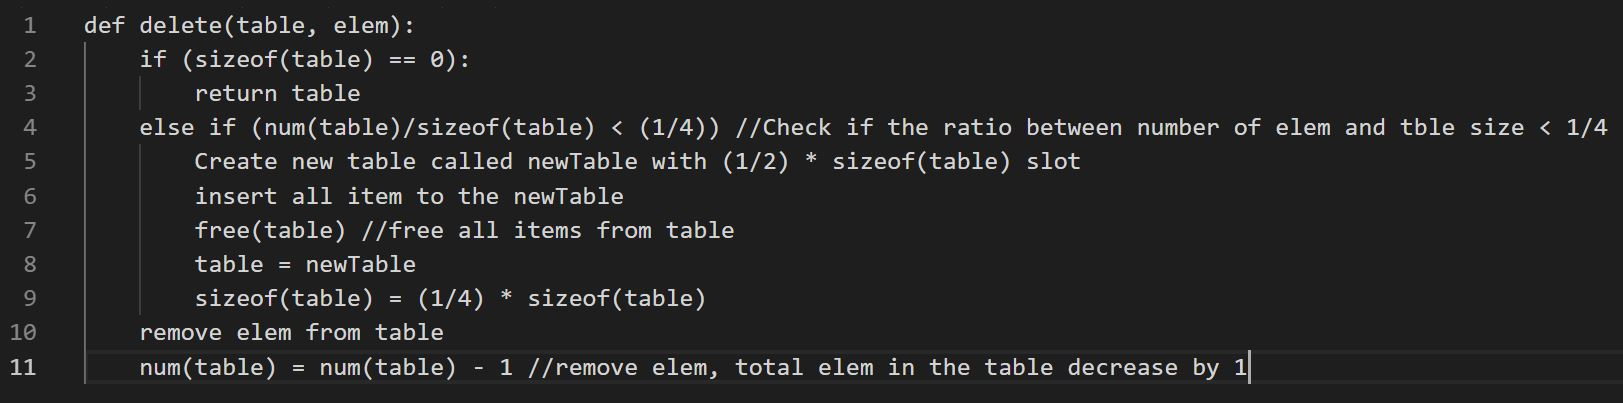
\includegraphics[width=\textwidth]{q1.jpg}

\part{2}\\
By accounting method we going to assign value into each operation inside the function.\\
Let elem be an elem needed to be delete and table be a table containing elem.\\
Charge \$2 per deletion of elem:\\
\$1 pays for the deletion of elem\\
\$1 pays for an emptying slot\\
WLOG, let assume that the table with size of k has no credit left in any slot and there is $\frac{k}{2}$ amount of item inside the table. Let m be the number of slots that contain items, when we perform a deletion of elem we pay \$2. One is use for deletion and another is save for each item in the slots. When our load factor < $\frac{1}{4}$ we create a new table of size $\frac{k}{2}$. Then we copy the element from the old table to the new table. As we save \$1 for each non-empty slots, there would be enough credit to copy $\frac{k}{4}$ amount of item to a new table. This means there is no credit left over and the total credit will never be negative value.
\question{2}{Problem2}
Claim: set-partition is MP-complete\\
set-partition $\in$ NP:\\
Given $A \subseteq S$ where A is a set of numbers and S which is also a set of number.\\
We can create a verifier to check if the solution run in polynomial time using and algorithm below.\\
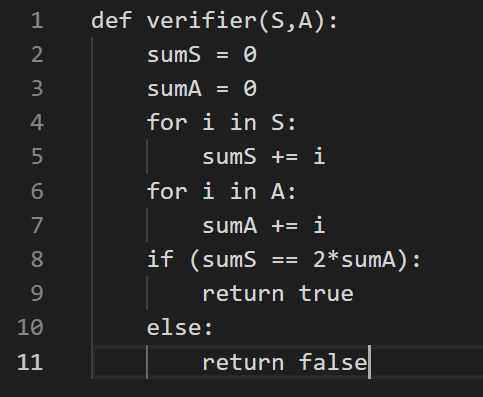
\includegraphics[width=\textwidth]{q2.jpg}\\
This algorithm time complexity is O(n). This is because we have 2 for-loops each run to all the elements in each set (line 4 and line 6). Let n be the length of S and m be the length of A. Other steps inside a loop take O(1). Instantiating an element in line 2 and 3 also take O(1). So $O(m \cdot 1) + O(n\cdot 1) 2 \cdot O(1) = O(n)$. As n id greater than m. $\lim_{n \to \infty} \frac{n}{n} = 1$. This mean it is in $\Omega(n)$ which means it is O(n).\\
set-partition is NP-hard:\\
By reducing set-partition to sub-set sum. subset-sum is a known NP problem that an instance $<A,t>$ will be computed in polynomial time complexity.\\
Let subset-sum be the summation of S, now we claim that:\\
$subset-sum \leq_{p} set-partition$\\
Claim: C is a solution for subset-sum $\iff $  D is a solution for set-partition\\
($\Rightarrow$) Suppose C is a solution in subset-sum where C takes A and S. We know that set A and a target $\frac{subset-sum}{2}$. S can be partition into set A and A' where A' = S - A. This then form a set-partition solution for S.\\
($\Leftarrow$) Suppose D is a solution in set-partition which takes S and A. Set A is a set that sum to a number in which when we double it, it equals the the sum of S. Which is a subset-sum solution when it takes A as an input with a target $\frac{subset-sum}{2}$.
\question{3}{Problem3}
Claim: Efficient-Recruiting is NP-Complete\\
Efficient-Recruiting $\in$ NP:\\
Given setK $\subseteq$ setM where setM is a set of all counselor and setK is a subset of setM.\\
Let map be a map of sports to $key_{i}$ ans $set_{i}$ which is a subset of applicant in setM.\\
We can create a verifier that take setK ans Map as an input to check if the solution is in polynomial time using an algorithm below.\\
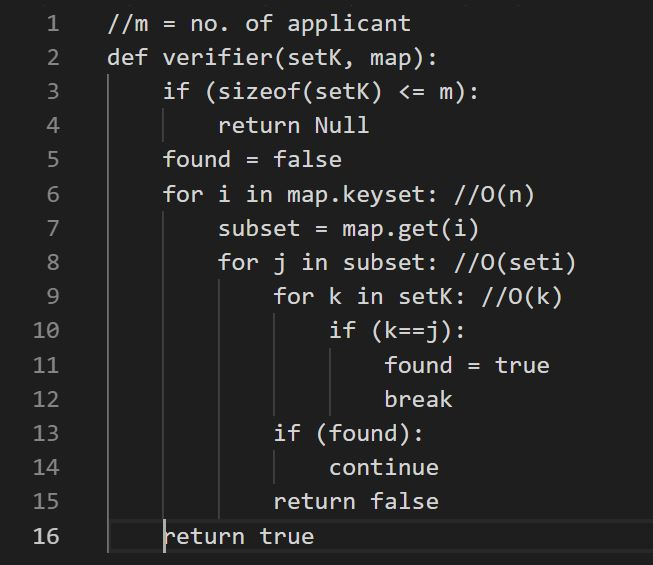
\includegraphics[width=\textwidth]{q3.jpg}\\
The running time is:
$$\sum_{i=0}^{n-1} set_{i} = O(n^{2}k)$$\\
Where n is the total number of element in map.
Efficient-Recruiting is NP-hard:\\
By reducing Efficient-Recruiting to vertex-cover. Vertex-cover for a graph G is a subset of vertices that covers all the edges in E. Let s be a size of counselors, the instance $<G,s>$ will be computed in polynomial time.\\
In order to remove this into a vertex-cover we needs to create a graph from Efficient-Recruiting problem. Let G be an undirected graph G = (V,E), where V are vertices and E are edges. Given M as a counselors vertices in V and N as a sports vertices in V, $i_{th}$ vertices are connected to all vertices in M. Assumes there is at least one edge in every vertex in N that connects to vertex in M. $\bar{G} = (V-M'), \bar{E})$ where $\bar{E}$ are edges after M' is removed from V to create $|V-M'| = k$ which is the counselors we will be hiring.\\
$Vertex-cover \leq_{p} Efficient-Recruiting$\\
Claim: C is a solution for vertex-cover $\iff$ D is a solution for Efficient-Recruiting\\
($\Rightarrow$) Suppose C is a solution in vertex-cover of instance $<G,k>$. This mean for $k = |M| - |M'|$ we can form a vertex cover of size k and every edges are covered within it. This then form an Efficient-Recruiting solution for N sports and at most k counselors.\\
($\Leftarrow$) Suppose D is a solution in Efficient-Recruiting of instance $<\bar{G},k>$, this means $\bar{G}$ has at least one edge in N connecting to a vertex in $V-M'=V'$ and the size V' is k. From the solution, $\bar{G}$ can use V' vertices to connect to all vertices and can cover all the edges in $\bar{E}$. Which then forms a vertex-cover solution for graph $\bar{G}$ with a vertex cover of size k.
\end{document}

